\section{Motivation}
{Die Ausgaben für das Internet der Dinge (IoT) wird weltweit, laut Statista, bis zum Jahr 2022 auf 1000 Milliarden US-Dollar steigen. Im Vergleich zum Jahr 2019 bedeutet dies, eine Steigerung von über 40\%.}\cite{STATISTA01:IOT} Bei einem solch starken Trend in der Informatik-Branche sollten sowohl Studenten, als auch Professoren dessen Grundlagen kennen.
Deshalb ist im Rahmen des Faches Softwarearchitektur an der technischen Hochschule Rosenheim diese Ausarbeitung geschrieben worden. Das Ziel ist es OpenHAB, ein Heimautomatisierungs-Tool, aus praktischer und technischer Sicht zu untersuchen. Außerdem wird dabei auf die Aspekte Markttauglichkeit und Benutzbarkeit in der Praxis eingegangen.

\section{Was ist OpenHAB?}
OpenHAB ist eine technologie-unabhängige Open-Source-Automatisierungssoftware für Smart-Homes.
Das Projekt wurde von Kai Kreuzer 2010 erstmals initiiert und wird mittlerweile durch die Community weiterentwickelt. Die Software ist hauptsächlich in Java und der Auszeichnungssprache XML geschrieben. Seit dem 16. Dezember 2019 ist die Version 2.5 erhältlich.\\
\\
Auf der offiziellen Website von OpenHAB \url{https://www.openhab.org/} sind drei klare Hauptziele definiert, die diese Software erreichen soll. Dabei ist ein Ziel die Plattformunabhängigkeit. Somit kann OpenHAB sowohl auf Linux, MacOS oder Windows betrieben werden. Auch das Hosten mit Docker oder einem Raspberry Pi wird unterstützt.\\
Weiterhin soll es durch die Plugin-Architektur möglich sein, fast jedes Gerät zu integrieren.
Es werden über 200 Technologien und mehrere tausende verschiedene Geräte unterstützt.\\
Das dritte Ziel weißt auf die vielen verschiedenen Automatisierungsmöglichkeiten hin, die OpenHAB zu bieten hat. Dabei werden Auslöser (in englisch: Trigger), Aktionen, Skripte und auch Voice-Kontrolle genannt.

\section{Bewertung OpenHAB}
In diesem Kapitel wird das open-source Projekt OpenHAB untersucht und bewertet. Das Projekt OpenHAB befindet sich auf Github unter \url{https://github.com/openhab/openhab-core}. Die hierfür verwendeten Kriterien sind orientiert an der QAware Open Source Quick-Check Liste.
Dies beinhaltet:
\begin{longtable}{| p{3cm} | p{12cm}|}
	\hline
	\textbf{Kriterium} & \textbf{Beschreibung} \\
	\hline \hline
	\centering Lizenz & Für welche Zwecke kann das Projekt genutzt werden? \\
	\hline
	\centering Reifegrad & Existiert eine stabile Version > 1.0?  \\
	\hline
	\centering Support & Existiert Issue-Tracking und ein Antwortzeit auf Tickets unter 24h? \\
	\hline
	\centering Dokumentation & Existiert?
	\begin{itemize}
		\item Api-Dokumentation
		\item Getting Started Tutorial
		\item Aktuelle Dokumentation
	\end{itemize} \\
	\hline
	\centering Projekt Aktivität & Gibt es?
	\begin{itemize}
		\item Mindestens 1 Release im letzten Jahr
		\item Mindestens 3 aktive Contributer
		\item Stetige Commit-Aktivität von mindestens 1x pro Monat
	\end{itemize}\\
	\hline
	\centering Bekanntheitsgrad & Vergleich von öffentlichem Interesse in Blockposts, auf Stackoverflow et cetera. \\
	\hline
	\caption{OpenHAB Projektbewertungskriterien}
	\label{table:openhub-judgement-kriteria}
\end{longtable}



\begin{itemize}
	\item \url{https://www.openhub.net/p/openhab}
	\item Was ist Openhub: Website zur Katalogisierung von open-source Softwareprojekten
	\item Dabei werden Daten wie Projektname, Beschreibung und Sourcecode erfasst. Basierend auf diesen Daten erstellt Open Hub eine Statistik, die es ermöglicht, Codeanalyse, Projektmitarbeiter, Aktivitäten und eine Übersicht zu erhalten. Dabei werden auch viele weitere open source Projekte miteinander verglichen um aussagekräftige Statistiken und Aussagen treffen zu können.
	\begin{itemize}
		\item openhub bewertet das Projekt mit sehr hoher Aktivitätsrate
		\item über 1.5 Millionen lines of code Hauptsächlich Java und XML
		\item 31\% des Codes ist dokumentiert (was soviel wie andere durchschnittliche Java-Projekte ist)
		\item insgesamt 1140 Contributers und 20k commits
		\item Basierend auf dem Vergleich von Commits des Vorjahres und des jetzigen Jahres, steigt das Interesse in OpenHAB
		\item Im letzten Jahr waren es 343 neue Contributer. Das macht OpenHAB zu einem der größten open source-teams der Welt. Sie sind unter den top 2\% von allen Projektteams auf Openhub.
	\end{itemize}
	\item Lizenz: freie Software Lizenz EPL-2.0: ermöglicht kommerzielle und private Nutzung, Modifizierung, Weiterverbreitung. \url{https://www.eclipse.org/legal/epl-2.0/}
	\item Stable Release 2.5 > 1
	\item Durchschnittliche Antwortzeit in der Community > 24h? ja: wie beweisen?
	\item OpenHAB wurde bereits in der Bachelorarbeit von Pirmin Gersbacher vom Jahr 2017/2018 anhand von usecases untersucht und verglichen. Im Vergleich stellte sich folgende Ergebnistabelle \ref{fig:comparison-openhab}\cite{BA01:OPH} heraus.
\end{itemize}

\begin{minipage}{\textwidth}
	\centering
	\captionsetup{type=figure}
	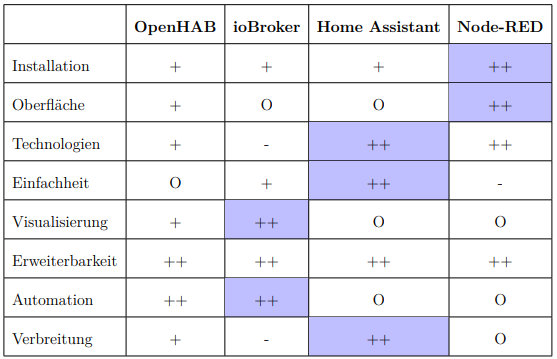
\includegraphics[width=0.8\textwidth]{\figdir/comparison-openhab.PNG}
	\caption{Vergleich OpenHAB und anderen Heimautomatisierungstools von 2017/2018 \label{fig:comparison-openhab}}
\end{minipage}


\section{Datenintegriertät und Sicherheit}
\url{https://www.openhab.org/docs/installation/security.html}
\begin{itemize}
	\item Through the command line console, which is done through SSH and thus always authenticated and encrypted. You will find all details about this in the Console documentation.
	\item Through HTTP(S) over \url{https://<ip>:8443}
	\item Options for Secure Remote Access
	\begin{itemize}
		\item VPN: The most secure option is probably to create a VPN connection to your home network
		\item myopenHAB Cloud Service with a tunnel that forwards all requests to the openHAB instance
		\item Running openHAB Behind a Reverse Proxy: A reverse proxy simply directs client requests to the appropriate server. This means you can proxy connections to \url{http://mydomain_or_myip} to your openHAB runtime.
	\end{itemize}
\end{itemize}



\section{OpenHAB aus technischer Sicht}
In diesem Kapitel sind die grundlegenden Komponenten, die OpenHAB verwendet, tabellarisch dargestellt. Anschließend wird detaillierter auf die einzelnen Elemente eingegangen und wie diese miteinander in Beziehung stehen. Ein Weiterer Aspekt von OpenHAB kommt in diesem Kapitel immer wieder zum Vorschein. OpenHAB sieht nicht den einen Weg vor etwas zu installieren/einzubinden. So kann z.B. je nach vorliebe des Nutzers eine Geräte über die Web-Oberfläche integriert werden, als auch programmatisch in dafür vorgesehen Datei-ORdner als Code. Dieses Konzept findet sich immer wieder z.B. für Bindings, Things, Items, Rules usw. OpenHAB liefert für das Entwickeln von Add-Ons Skelleton-Skripte, welche die von openHAB bentigte Struktur erzeugen. Für manuelles Hinzufügen von Things, Items, Rules usw. bietet openHAB bereits eine ORdnerstruktur. Diese ist so offensichtlich, dass es trivial ist zu entscheiden, wo welche Komponente hinzugefügt werde soll. Sollte dies dennoch unklar sein, wird der Nutzer noch weiter durch readme-dateien unterstützt. Siehe 
\captionsetup{type=figure}
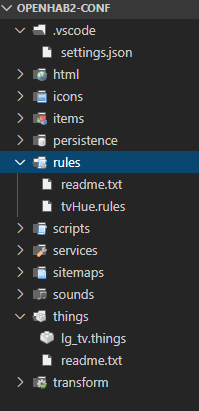
\includegraphics[width=0.25\textwidth]{\figdir/openHab-conf-folder-structure.png}
\caption{openHAB-conf Ordnerstruktur \label{fig:openHab-conf-folder-structure}}

\begin{longtable}{| p{2cm} | p{13cm}|}
	\hline
	\textbf{Konzept} & \textbf{Beschreibung} \\
	\hline \hline
	\centering Add-ons & Erweiterung welche von openHab ermöglicht werden. \\
	\hline
	\centering Bindings & openHAB-Komponenten, welche die Schnittstelle zu fremd Systemen bereitstellen.  \\
	\hline
	\centering Things & erste von openHAB (Software) generierte Darstellung von Geräten. \\
	\hline
	\centering Channels & openHAB (Software)-Verbindung zwischen "`Dingen"' und "`Gegenständen"'. \\
	\hline
	\centering Items & von openHAB (Software) generierte Darstellung von Informationen über die Geräte.\\
	\hline
	\centering Rules & führen automatische Aktionen durch (in einfachster Form: wenn "`dies"' passiert, wird openHAB "`das"' tun).\\
	\hline
	\centering Sitemaps & ist die von openHAB (Software) generierte Benutzeroberfläche (Website), die Informationen präsentiert und Interaktionen ermöglicht.\\
	\hline
	\caption{OpenHAB Komponenten}
	\label{table:openhub-components}
\end{longtable}

\subsection{Add-ons}
openHAB sich selbst als System bezeichnet welches alles Integriert, dies wird dadruch erreicht, dass es von der so konzipiert ist, dass bestimmte bereiche jederzeit erweitert werden können. OpenHAB gibt hier als verschiedene Module/Komponenten, welche neu hinzugefügt werden können vor.
\begin{itemize}
	\item Bindings
	\item Automation Engine Modules
	\item Transformations / Profiles
	\item IO Services
	\item Persistence Services
	\item Audio \& Voice
\end{itemize}
Um nicht den Rahmen dieser ARbeit zu übersteigen wird Detailierter auf Bindings eingegangen. Was unter anderem daran liegt, dass Die Dokumentation von openHAB, welche die entwicklung von IO-, Persistence Services und Audio/Voice mit einem TODO beschreibt eher dürftig ist. Bei den Transforamtions / Profiles handelt es sich um transformationen welche genutzt werden können um zu übertragenede Werte durch einen Channel zu manipulieren/tranformieren.
Add-ons sind in openHab das Herzstück der pluggable Architecture. Da Nutzer des Systems ihre individuellen Bedürfnisse haben und sich demnach nciht alle verfügbaren Add-ons installieren müssen, sondern nur diejenigen welche für Ihre Bedürfnisse nötig sind. Sollte es allerdings keine passendes Add-on für ein gewünschtes Gerät geben, steht der erweituerng und dem entwicklen eines eigenenen Add-ons durch das Add-on System nichts im Weg. Mehr noch, durch den OpenSource gedanken, welcher openHAB vorantreibt könnte das Gesamt-System durch ein weiteres Add-on erweitert werden. 

\subsection{Bindings}
Bindings sind die Schnittstelle bzw. die Erweiterung, welche es erst ermöglicht andere Systeme mit openHAB zu integrieren. Mit einem Binding kann sowohl ein Pysisches Geräte z.B. eine LG Fernseher als auch eine Service z.B. Spotify angebunden werden. Die Bindings sind dabei soweit abstrahiert, dass nicht jedes einzelne Model bzw. Version eine eigenes Binding benötigt.
Ein Binding ermöglicht es dem System erst neue Geräte im System zu erkennen. Und diese als Thing im openHAB System zur weiteren Interaktion zur Verfügung zu stellen. Interessant ist hierbei, dass Bridges oder Schnittstellen wie Bluetooth es erst ermöglichen Weitere Geräte zu erkennen. So kann durch das Hue-Binding die Hue-Bridge integriert werden, welche es wiederum ermöglicht einzelne Komponenten des Hue-Systems anzusprechen (Lampen), welche nicht direkt erkannt und angesporchen werden konnten.
Laut openHAB gibt es aktuell über 300 Bindings und dadurch können über 2000 Things angesprochen werden.
OpenHab bietet zusätzlich zur Dokumentation noch Untestützung für das Entwickeln eines Eigenen Bindings durch eine Skeletton skript, welches die Stuktur eines Bindings inklusive Beispielen und Erklärungen welche Methonde/Funktionen wie gestaltet werden müssen und was diese Tun. Siehe:
\captionsetup{type=figure}
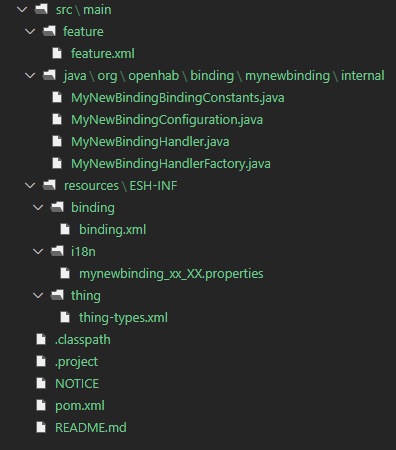
\includegraphics[width=0.5\textwidth]{\figdir/own_binding_skeletton.png}
\caption{Skelett für Binding \label{fig:own_binding_skeletton}}


\subsection{Things}
Things sind die repräsentation von Geräten/Services innerhalb des Systems. Berachtet man die Objektorierntierung ist es ein sehr schönes Beispiel wie im einem Computersystem ein realer gegenstand beschreiben werden kann.
Things bieten verschiedene so gennante Channels an. Diese entsprechen die Funktionen/Aktionen welche das Gerät ausführen kann.
Things können auf 3 verschiedene arten openHAB hinzugefügt werden
\begin{itemize}
	\item per Web-Oberfläche per Button click in der Inbox, nachdem das entsprechende Binding installiert wurde. Hierbei werden alle nötigen Einstellungen für das Thing automatisch getroffen. Diese können nachträglich noch bearbeitet werden z.B. Bezeichnung. 
		\captionsetup{type=figure}
		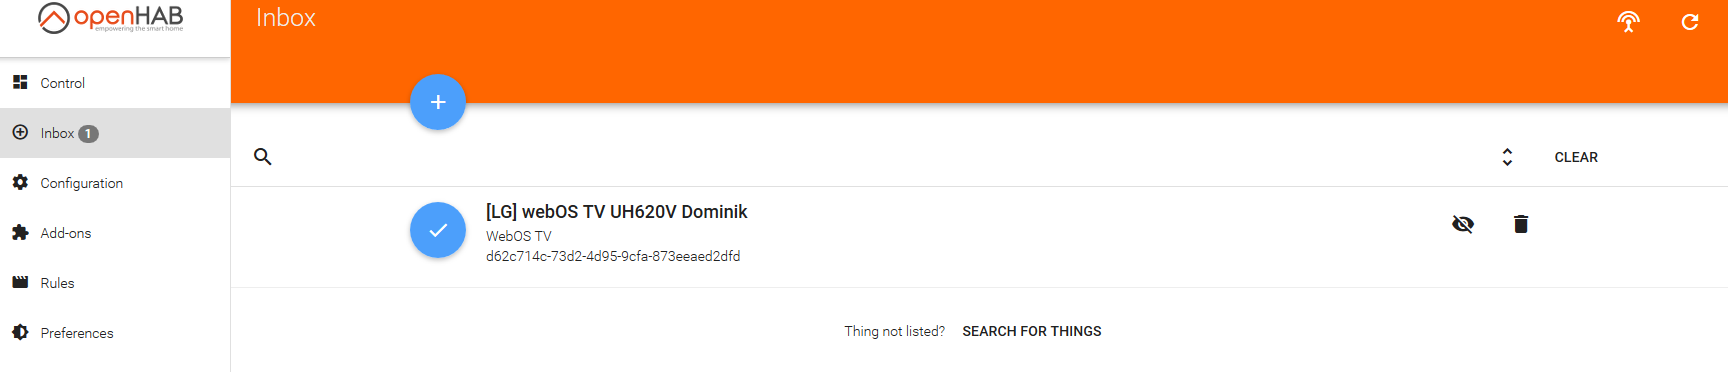
\includegraphics[width=1\textwidth]{\figdir/thing_add.png}
		\caption{Thing per Paper-UI \label{fig:thing-add-paper-ui}}
		
	\item per Web-Oberfläche Manuell. Erlaubt völlige Einstellung im Vorhinein. Allerdings ist auf Statische IP-Adressen zu achten.
		\captionsetup{type=figure}
		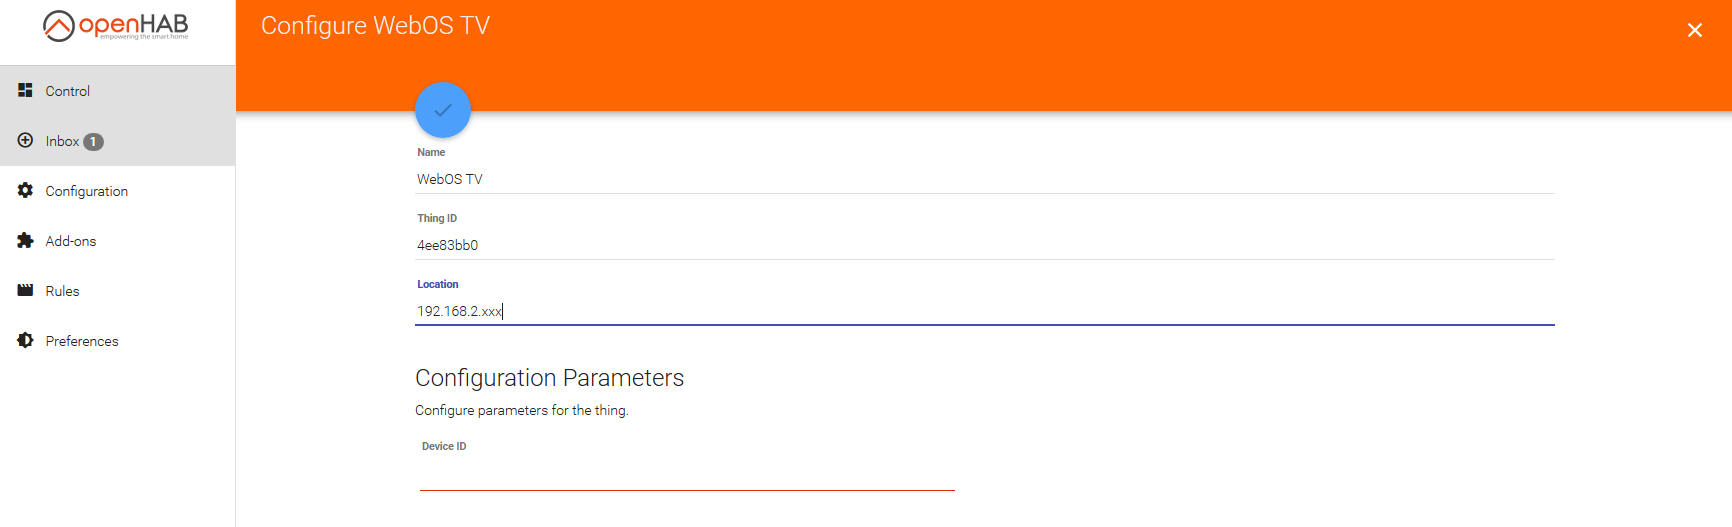
\includegraphics[width=1\textwidth]{\figdir/thing_add_manuel.png}
		\caption{Thing per Paper-UI Manuell \label{fig:thing-add-paper-ui-manuel}}
		
	\item per Code. Ermöglicht und benötigte komplette manuelle eingabe aller nötiger Infomrmationen wie IP-Adresse
		\captionsetup{type=figure}
		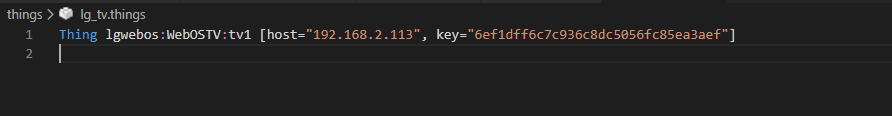
\includegraphics[width=1\textwidth]{\figdir/thing_add_code.png}
		\caption{Thing per Code \label{fig:thing-add-code}}
\end{itemize}

\subsection{Channels}
sind Kommunikationswege welche von den Things angeboten werden. Channels verbinden Things und Items. Und könne in openHab, bzw. den Rules genutzt werden. Sie stellen die Verbindung von externen Gerät zu openHAB aktionen dar. Über die Channels können Informationen durch PAramerter ausgetauscht werden. So wäre z.B. die Helligkeit einer Lampe ein Parameter, welcher durch einen Channel übertragen werden kann. nicht jedoch die Informationen, dass sich die Helligkeit ändern soll. Hierfür wird das Item benötigt, welches durch den Channel an das Thing verbunden wrude.

\subsection{Items}
Der Begriff Item wirkt unter umständen falsch. Ein Item könnte auch als Aktion beschreiben werden. Ein Item selbst hat sehr wenig Informationen. Das Item besteht neben eine Titel noch aus eine Kategorie und eine Gruppe um es zuzuordnen und um gleichzeitig mehrere Items gleichzeitig anzusteueren.. Außerdem hat ein Item noch einen Typ, dieser Typ entspricht einer Menge von Basistypen, welche von openHAB angeboten werden. Diese sind unter anderem String, Numnber, DateTime, Location, Player usw. \url{https://www.openhab.org/docs/configuration/items.html#type}.
Wichtig ist auch der Status. Wodoruch es doch wieder ein Item anstatt einer Aktion ist. (könnte man item als object bezeichnen mit label, kategorie, status und nur einer funktion??? memo an mich DAM)
Items sind essentielle bestandteile um das Panel zu bauen, da die Widgets über Items mit den Geräten agieren.


\begin{lstlisting}[language=java,firstnumber=1,caption=Item-Gruppierung Beispiel,label=lst:group-items]
	Group groundFloor
	Switch kitchenLight (groundFloor)
	Switch livingroomLight (groundFloor)
\end{lstlisting}

\subsection{Rules}
\begin{itemize}
	\item Rules stelln wenn dann Beziehungen dar
	\item Diese können sowohl über zusammenklicken, als auch programmatisch erstellt werden. 
	\item Das Zusammenklicken basiert auf einem noch nicht fertigen Feature namens experimental rules. Zum Zeitpunkt dieser Arbeit können dadurch schon einige Standardrules definiert werden. Allerdings fehlt beispielsweise noch die Vergleichsoption größer oder größer-gleich
	\item Codeblock \ref{lst:sample-rule} zeigt ein programmatisch erstellte Rule.
	\begin{itemize}
		\item Eine Rule besteht immer aus einem Namen, einer when-Bedinung und einem then Abschnitt.
		\item Name dient als Zuordnung
		\item When ist der Trigger bzgw. Auslöser der Aktion, welche im then Block definiert ist.
		\item Diese Rule prüft, ob die Lautstärke des Items (TV) Dominik\_volumen sich verändert hat.
		Wenn das der Fall ist, wird eine geprüft, wiehoch denn die aktuelle Lautstärke ist.
		Folglich wird bei unter 20 die Lampe gedimmt und bei über 20 die Lampe erhellt.
		\item Falls etwas nicht klappen sollte, können auch Debug-Ausgaben mit dem Kommando logDebug geschrieben werden.
	\end{itemize}
\end{itemize}

Automatisierung wir durch Rules/Scripte erreicht, welche in erster linie durch Programmieren erzeugt werden. Um Regeln zu erzeugen, wird eine einfache wenn/dann-Struktur verwendet. Diese Regeln können auf verschiedene Bedingungen "lauschen". So können die Trigger von Items, Member of, Time, System oder Things stammen. Genauer kann die Bedingung noch durch eine verschiedene Formen eingeschränkt werden wie z.B. received command [<command>],  received update [<state>] oder changed [from <state>] [to <state>] usw.
Wenn diese Bedingung erfüllt ist, wird im DANN-Pfad die Reaktion definiert. So können Item oder Ganze Gruppen angesprochen werden und durch diese über Channels Informationen weitergegeben werden.
Wie im Codebeispiel 2?? zu sehen, kann auch 
\begin{lstlisting}[language=java,firstnumber=1,caption=Beispiele Rule Beispiel,label=lst:sample-rule]
rule "React on Volume (LGWebOSTVUH620VDominik_Volume) change"
when
	Item LGWebOSTVUH620VDominik_Volume changed
then
	logDebug("React some changes on Volume", "some Message" + LGWebOSTVUH620VDominik_Volume.state.toString)
if ( LGWebOSTVUH620VDominik_Volume.state >= 20 ) {
	HueWhiteLamp2_Brightness.sendCommand(80)
}
else {
	HueWhiteLamp2_Brightness.sendCommand(5)
}
end
\end{lstlisting}

\subsection{Sitemaps}

\subsection{Api}
\url{https://www.openhab.org/docs/configuration/restdocs.html}
\begin{itemize}
	\item Item ein-/ausschalten
	\item Eine List von allen Items, Sitemaps ausgeben lassen
	\item Mit einem Editor auf die ganzen Komponenten zugreifen:
	\begin{itemize}
		\item Visual Studio Code installieren
		\item Openhab Extension installieren
		\item Geteiltes Openhab Laufwerk als Ordner öffnen
		\item Openhab Extension konfigurieren
		\item Es werden auch andere Editoren unterstützt
	\end{itemize}
\end{itemize}

\section{Verwendung von OpenHAB}
\subsection{Integration der Big Player}
\begin{itemize}
	\item Amazon Alexa und Echo Dot Integration möglich
	\begin{itemize}
		\item Alexa:
		\begin{itemize}
			\item This certified Amazon Smart Home Skill allows users to control their openHAB powered smart home with natural voice commands. Lights, locks, thermostats, AV devices, sensors and many other device types can be controlled through a user's Alexa powered device like the Echo or Dot.
			\item \url{https://www.openhab.org/docs/ecosystem/alexa/}
			\item \url{https://www.openhab.org/addons/bindings/amazonechocontrol/}
		\end{itemize} 
		\item Google Home
		\begin{itemize}
			\item Google Home Integration möglich
			\item With the Action you can voice control your openHAB items and it supports lights, plugs, switches and thermostats. The openHAB Action comes with multiple language support like English, German or French language.
			\item The openHAB Action links your openHAB setup through the myopenHAB.org cloud service to the Google Assistant platform
			\item openHAB Cloud Connector configured using myopenHAB.org . (Items DO NOT need to be exposed to and will not show up on myopenHAB.org
			, this is only needed for the IFTTT service!)
			Google account.
			Google Home or Google Home mini.
			
			\url{https://www.openhab.org/docs/ecosystem/google-assistant/}
		\end{itemize} 
	\end{itemize}
	
\end{itemize}

\subsection{Beispiel Aufbau eines OpenHAB Smart-Homes}
\begin{itemize}
	\item OpenHAB auf Raspberry Pi 3/4 installiert
	\item Welche Geräte haben wir mit OpenHAB verbunden?
	\begin{itemize}
		\item Spotify
		\begin{itemize}
			\item Lautstärkeregler
			\item Aktueller Song Display
		\end{itemize}
		\item LG Smart TV
		\begin{itemize}
			\item Lautstärkeregler
			\item An- und ausschalten
			\item One-Way-Chat
		\end{itemize}
		\item Lampen
	\end{itemize}
	\item Wie haben wir die Geräte verbunden?
	\begin{itemize}
		\item \textbf{Verschiedene Binding:}
		\item Spotify Binding
		\item LG Smart TV Binding
	\end{itemize}
	\item On the server the configuration is stored somewhere in userdata (/var/lib/openhab2 for apt-get installs).
	In an upgrade the userdata folder is preserved when using apt-get.
\end{itemize}
\begin{minipage}{\textwidth}
	\centering
	\captionsetup{type=figure}
	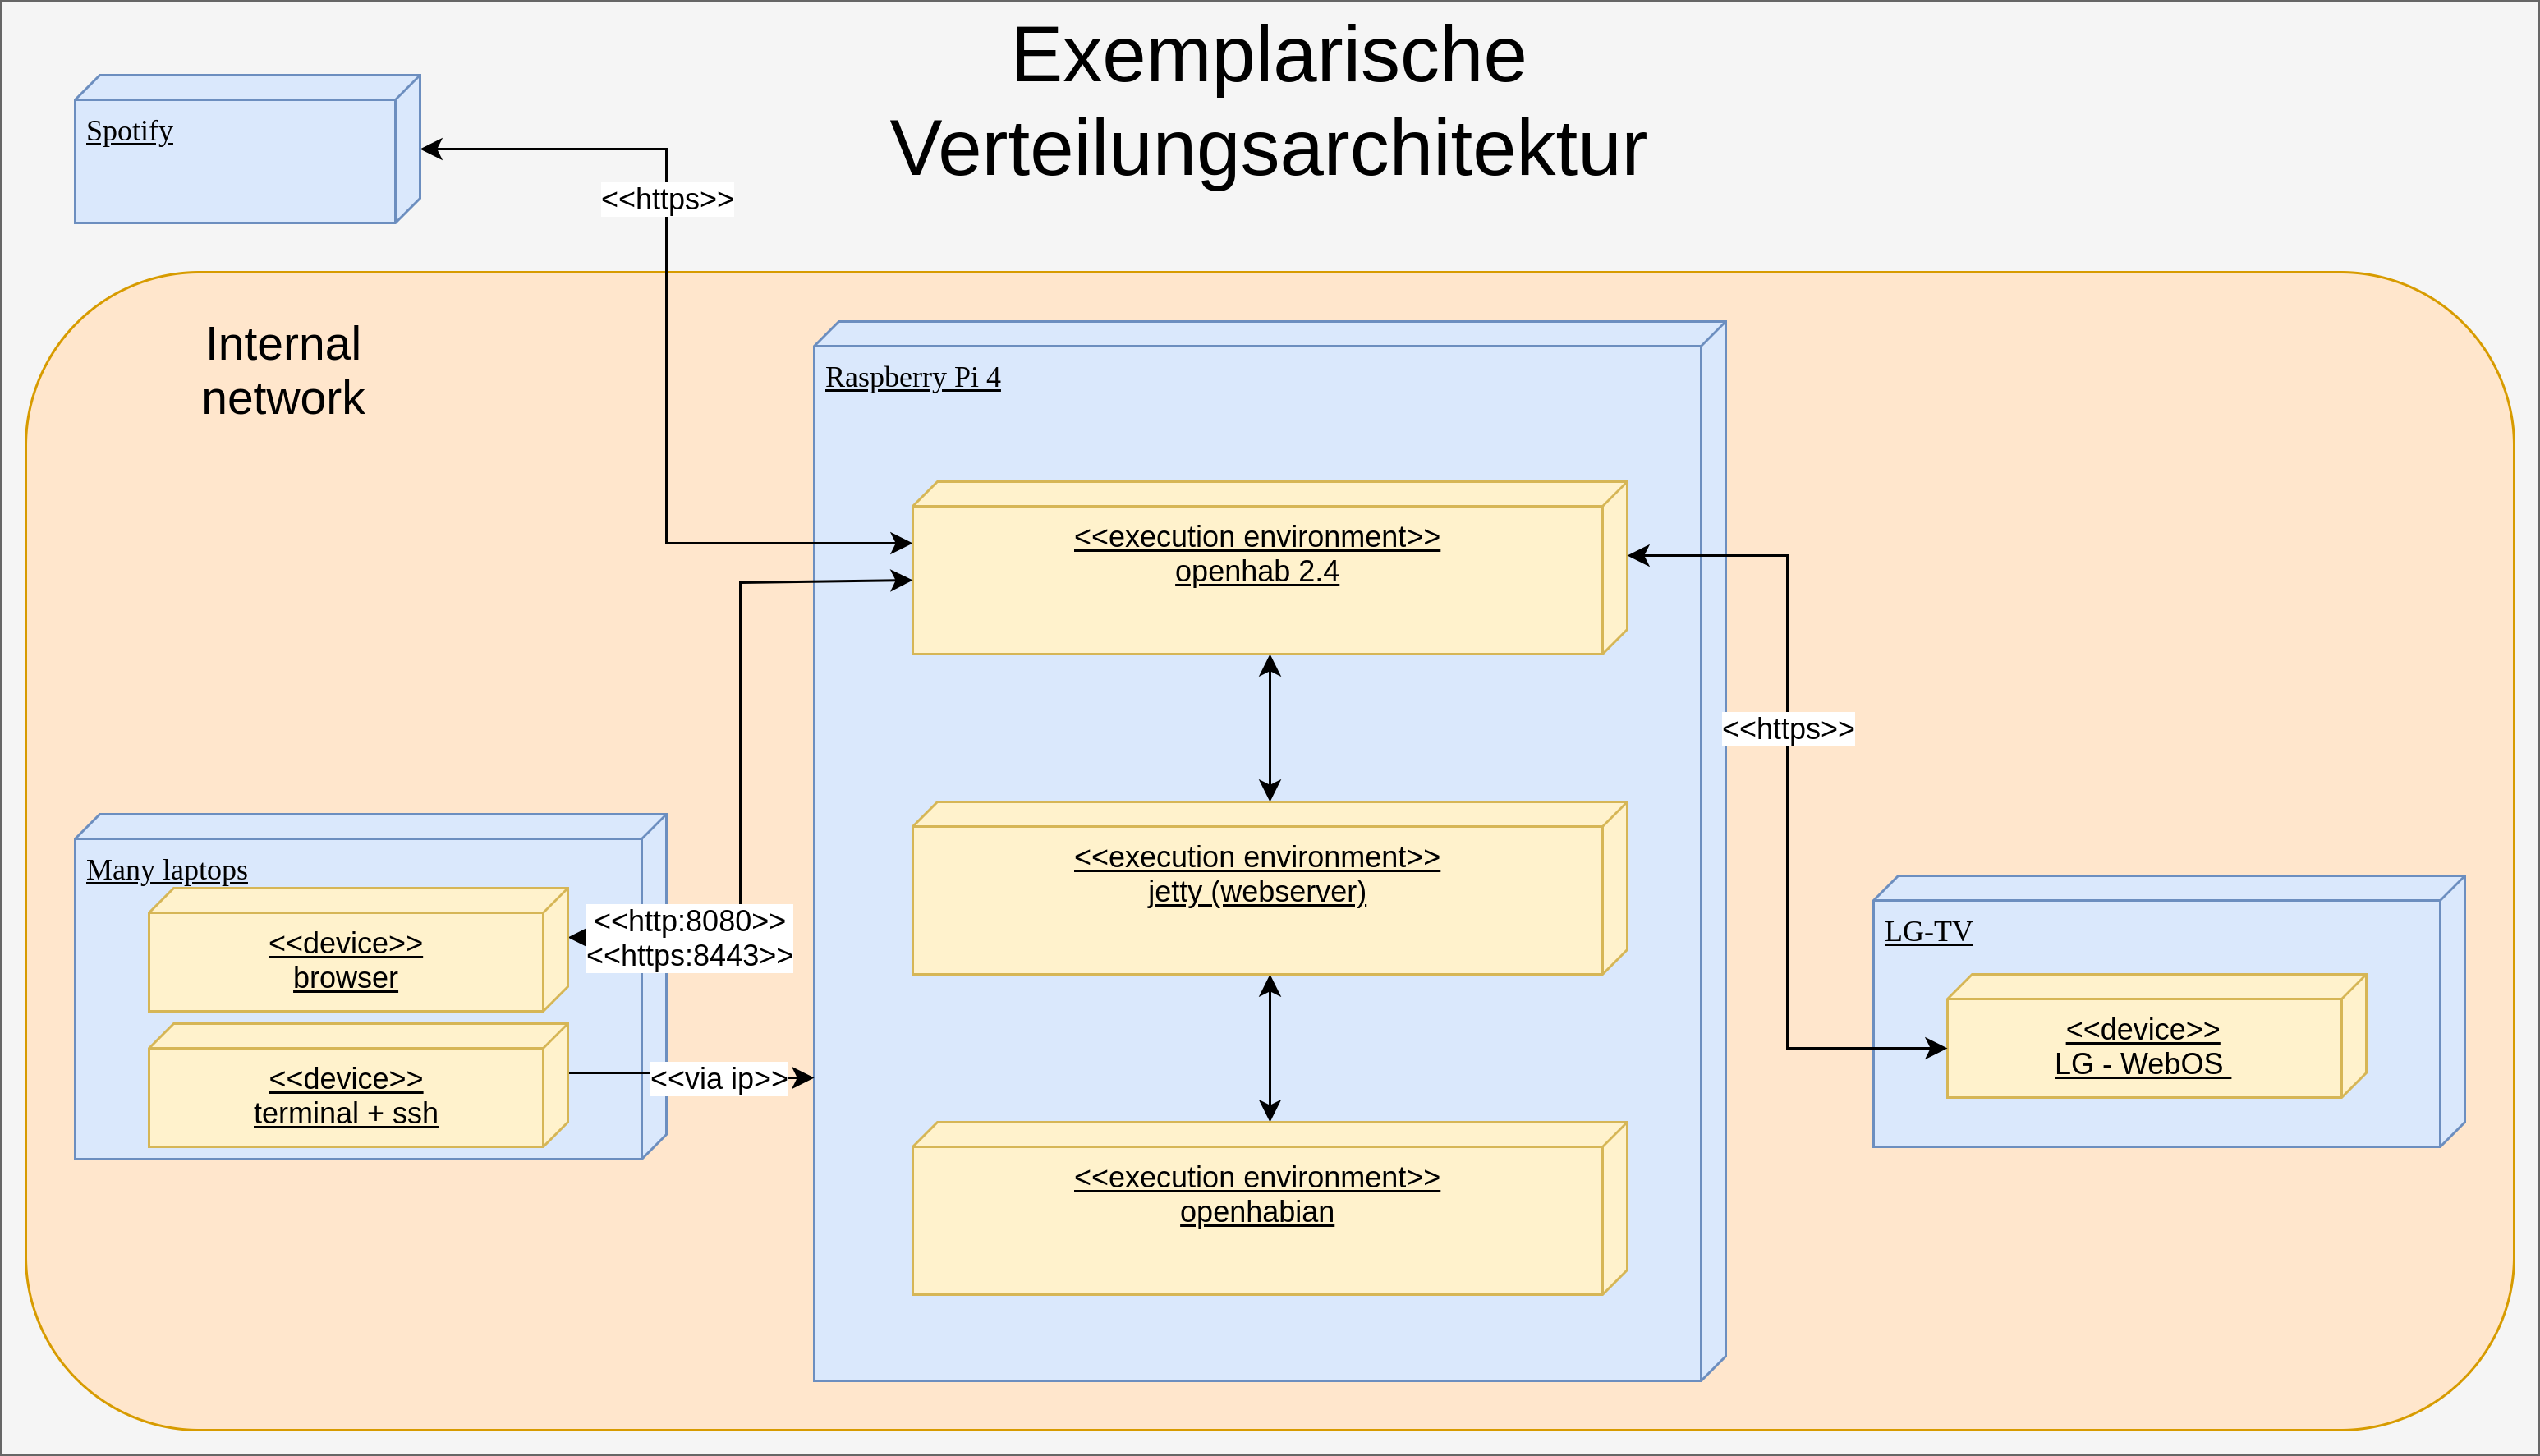
\includegraphics[width=1\textwidth]{\figdir/verteilungsarchitektur.png}
	\caption{Verteilungsarchitektur \label{fig:verteilungs-architektur}}
\end{minipage}
\begin{minipage}{\textwidth}
	\centering
	\captionsetup{type=figure}
	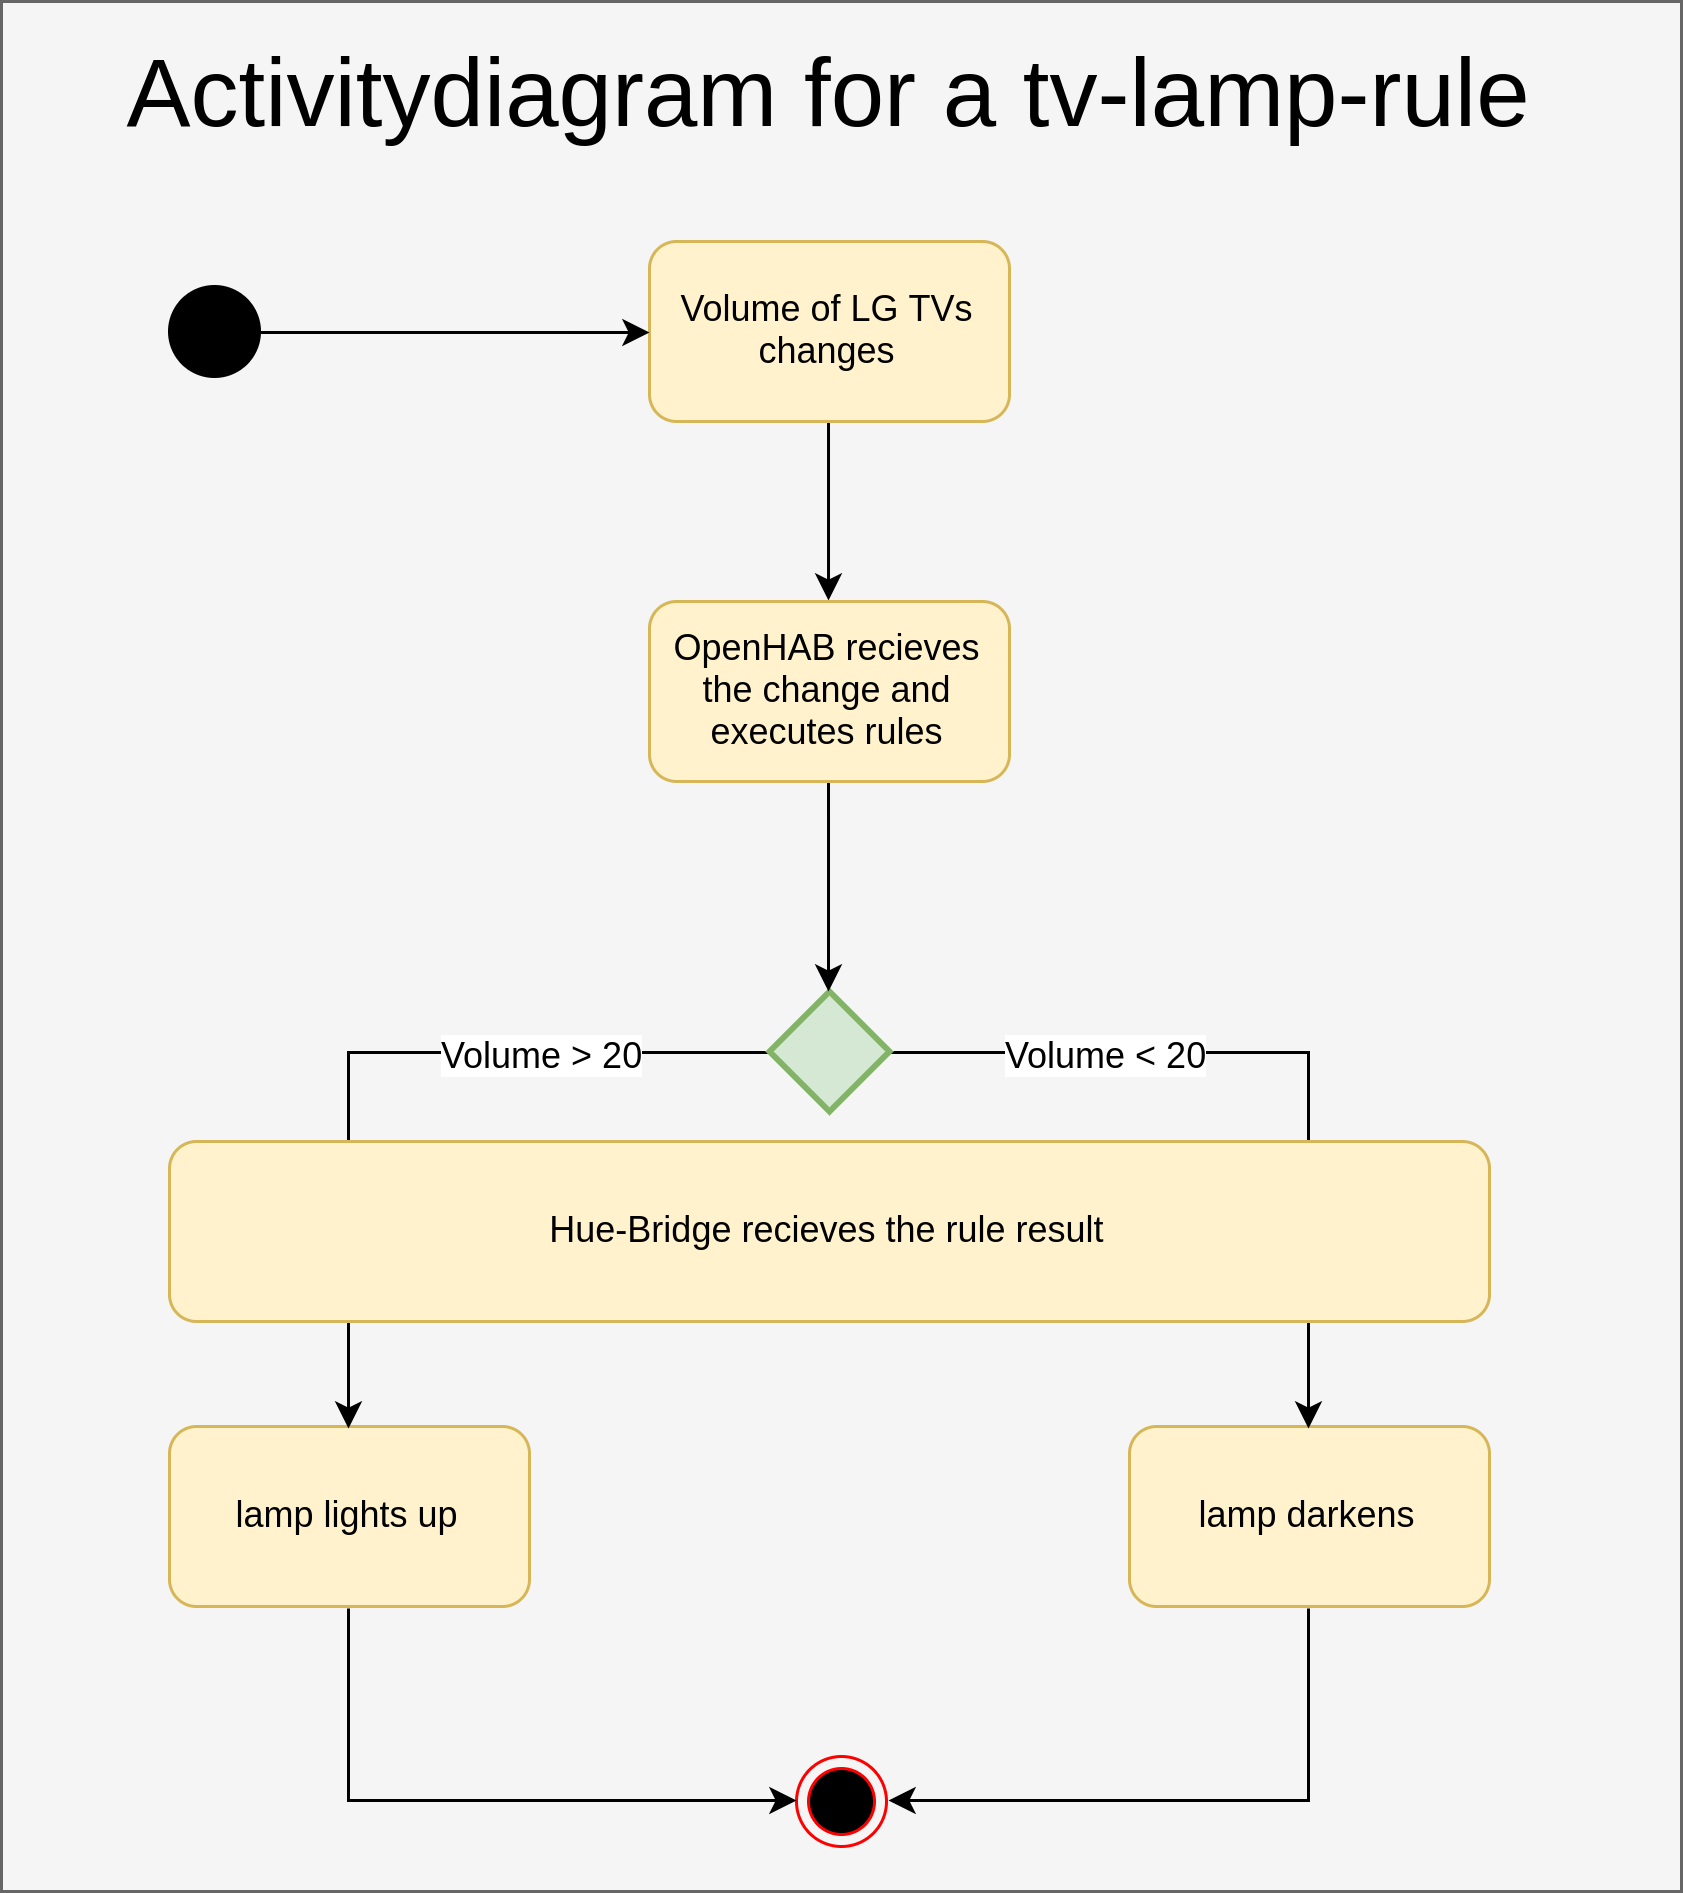
\includegraphics[width=1\textwidth]{\figdir/activitydiagram-lg-light-rule.png}
	\caption{Aktivitätsdiagram für eine Rule \label{fig:activity-diagram}}
\end{minipage}

\subsection{Umgang mit OpenHAB}
\begin{itemize}
	\item Das meiste klickt mans ich zusammen: Bindings, Rules, Channels, Items, Things
	\item Implementierung von rules scheint idiotensicher, weil:
	\begin{itemize}
		\item einfacher Syntax
		\item Abhängigkeiten managed Openhab
	\end{itemize}
	\item Bindings schreiben scheint eher schwieriger
\end{itemize}

\section{Fazit}
\subsection{Stärken}
Some of openHAB's strengths are:

Its ability to integrate a multitude of other devices and systems. openHAB includes other home automation systems, (smart) devices and other technologies into a single solution
To provide a uniform user interface and a common approach to automation rules across the entire system, regardless of the number of manufacturers and sub-systems involved
Giving you the most flexible tool available to make almost any home automation wish come true; if you can think it, odds are that you can implement it with openHAB.
\subsection{Schwächen}
\textbf{Wollen wir das hier als SWOT Analyse aufziehen?}
\begin{itemize}
	\item Integration von USB-Geräten scheint eher kompliziert. Vor allem auf Raspberry Pi
	\item Serial Binding wird nicht angezeigt
	\begin{itemize}
		\item Mikrofon an Raspberry Pi oder anderes Geräte verbinden
		\item Input des Mikrofons über OpenHAB an ein Ausgabegerät, wie zum Beispiel eine Bluetooth Box, senden und abspielen
		\item Raspberry hat da auch für große Probleme bei der Geräteerkennung gesorgt - USB gerät wurde nicht im devices Verzeichnis aufgeführt und somit konnte auch keine Verbindung mit OpenHAB aufgebaut werden
		\item OpenHAB Serial Device Binding wurde auch nicht angezeigt, um Geräte darüber zu suchen
	\end{itemize}
\end{itemize}

\section{Infos:}
\textbf{Ausgangslage}
Untersuchen Sie die Architektur und Features von OpenHAB und
schreiben Sie ein Beispielanwendung.
Mit myOpenHub existiert eine kostenlose Plattform die sie nutzen
können.

\textbf{Beantworten Sie dabei}
\begin{itemize}
 \item Aktueller Status des Projekts und  
 \item Integration der Big Player wie Alexa und Google Home
 \item Welche Tools und Konzepte und APIs gibt es
 \item Welche Deployment Modi und Betriebsmodi existieren
 \item Untersuchen Sie auch Aspekte wie Datenintegriertät und Sicherheit
\end{itemize}

\textbf{Unterlagen Linkes}
\begin{itemize}
	\item \url{https://www.myopenhab.org/}
	\item \url{https://www.openhab.org/}
	\item \url{https://jaxenter.de/openhab-2-4-78711}
\end{itemize}

%%% Local Variables: 
%%% mode: latex
%%% TeX-master: "thesis.tex"
%%% End: 
